%
		\subsection{2d3v PIC}\label{sec:pic_2d3v}
%
			In the following, I will highlight the difficult tasks of a spatially twodimensional PIC simulation, refering to the scheme in~\autoref{fig:picscheme}.
%
			\paragraph{Discharge Setup}%
			In the beginning of the simulation, before the first calculation step is done, the domain has to be constructed. The cylindrical setup is reduced to the radial and axial dimensions, e.g\@ $(r,z)$ for reasons of symmetry. The five-dimensional phase-space is completed with the full velocity triplet $\vec{v}=(v\ix{r},v\ix{z},v_{\vartheta})$. Two onedimensional grids in radial and axial directions, with $N\ix{r}$ and $N\ix{z}$ equally sized partitions respectively, are layered over each other to form the final discharge domain. Hence, the are of a single mesh cell is $\Delta r\ix{0}^{2}$. The spatial and temporal discretisation $\Delta r\ix{0}$ and $\Delta t\ix{0}$ are chosen to be dimensionless, so calculations inside the code can be performed much more easily and are less likely to have errors.\\
			Additionally, certain physical properties have to be scaled according to the spatial weight of a cell. Because a `quasi-three-dimensional' cell of coordinates $(n\ix{r},n\ix{z})$ grows in volume with increasing radial index (for a more visual approach, take a look at~\autoref{fig:radialcylinder}), a weighting factor needs to be multiplied with properties like densities and pressure.\\
			After the domain composition, the particle initialization is to be done. Here, one uses pressure and intial density to model a global distribution of electrons, ion and neutral species. The corresponding super particle factor is used to decrease computational time. Though it has been proven that this does not introduce artifacts to the simulations results --- the equation of motion only depends on a charge-to-mass-ratio --- it should not be too high. Collisions may be underrepresented when there are not enough targets, though in reality $\sim\tenpo{4}$ times the amount of particles would be available.\\
			To initialize the particles, a number of electrons, ions and neutrals is ditributed in each cell, using a Maxwell-distribution-function. Inside one mesh unit the, e.g\@ neutrals are spread continuosly and randomized. The same goes for the velocity, which is specified by the distribution function. The radial deformation of each cell has to be taken into acccount here. Therefore more particles have to be initiated in cells the closer they get to the outer limit of the cylindrical domain.\\
			Now that $N$ particles have been ditributed equally in the simulated area, the computational workload is shared between the $M\ix{PC}$ processing cores. The domain is therefore decomposed in partitions of equal particle numbers, e.g\@ $N/M\ix{PC}$. This speeds up the collisional and diagnostics routines, as each core only has to calculate on its own, but it does not reduce the time needed for the Maxwell's and Poisson's equation (see~\autoref{sec:picbasics}).
%
			\paragraph{Potential and Field Calculation}
			After the domain is filled and decomposed, the resulting density distribution, potential and electric field have to be calculated. The charges need to be mapped to the grid points to generate a density, which can be used by a discrete solver of the Poisson's equation (see~\autoref{equ:fivepointstar}). A linear weighting function is applied for each charge to form the density. The resulting scheme for a particle at $(r,z)$ in one and two dimensions is shown in~\autoref{fig:cicweighting} and~\autoref{equ:cicweighting}. The index tuple $k,j$ denotes the position in the twodimensional mesh, $n\ix{k,j}$ the corresponding density, $(r\ix{k},z\ix{j})$ the position --- this e.g\@ would be $r\ix{k}=\Delta r\ix{0}\cdot k$ and so on --- and $S\ix{k,j}$ the statistical weight, composed of dimensionless charge, super particle and volume factor. The quotient $A\ix{k,j}=\Delta r\ix{0}^{2}$ normalizes the result, so that no error is made when summarizing all four contributions of a single particle to the density.
%
			\begin{figure}
				\centering
				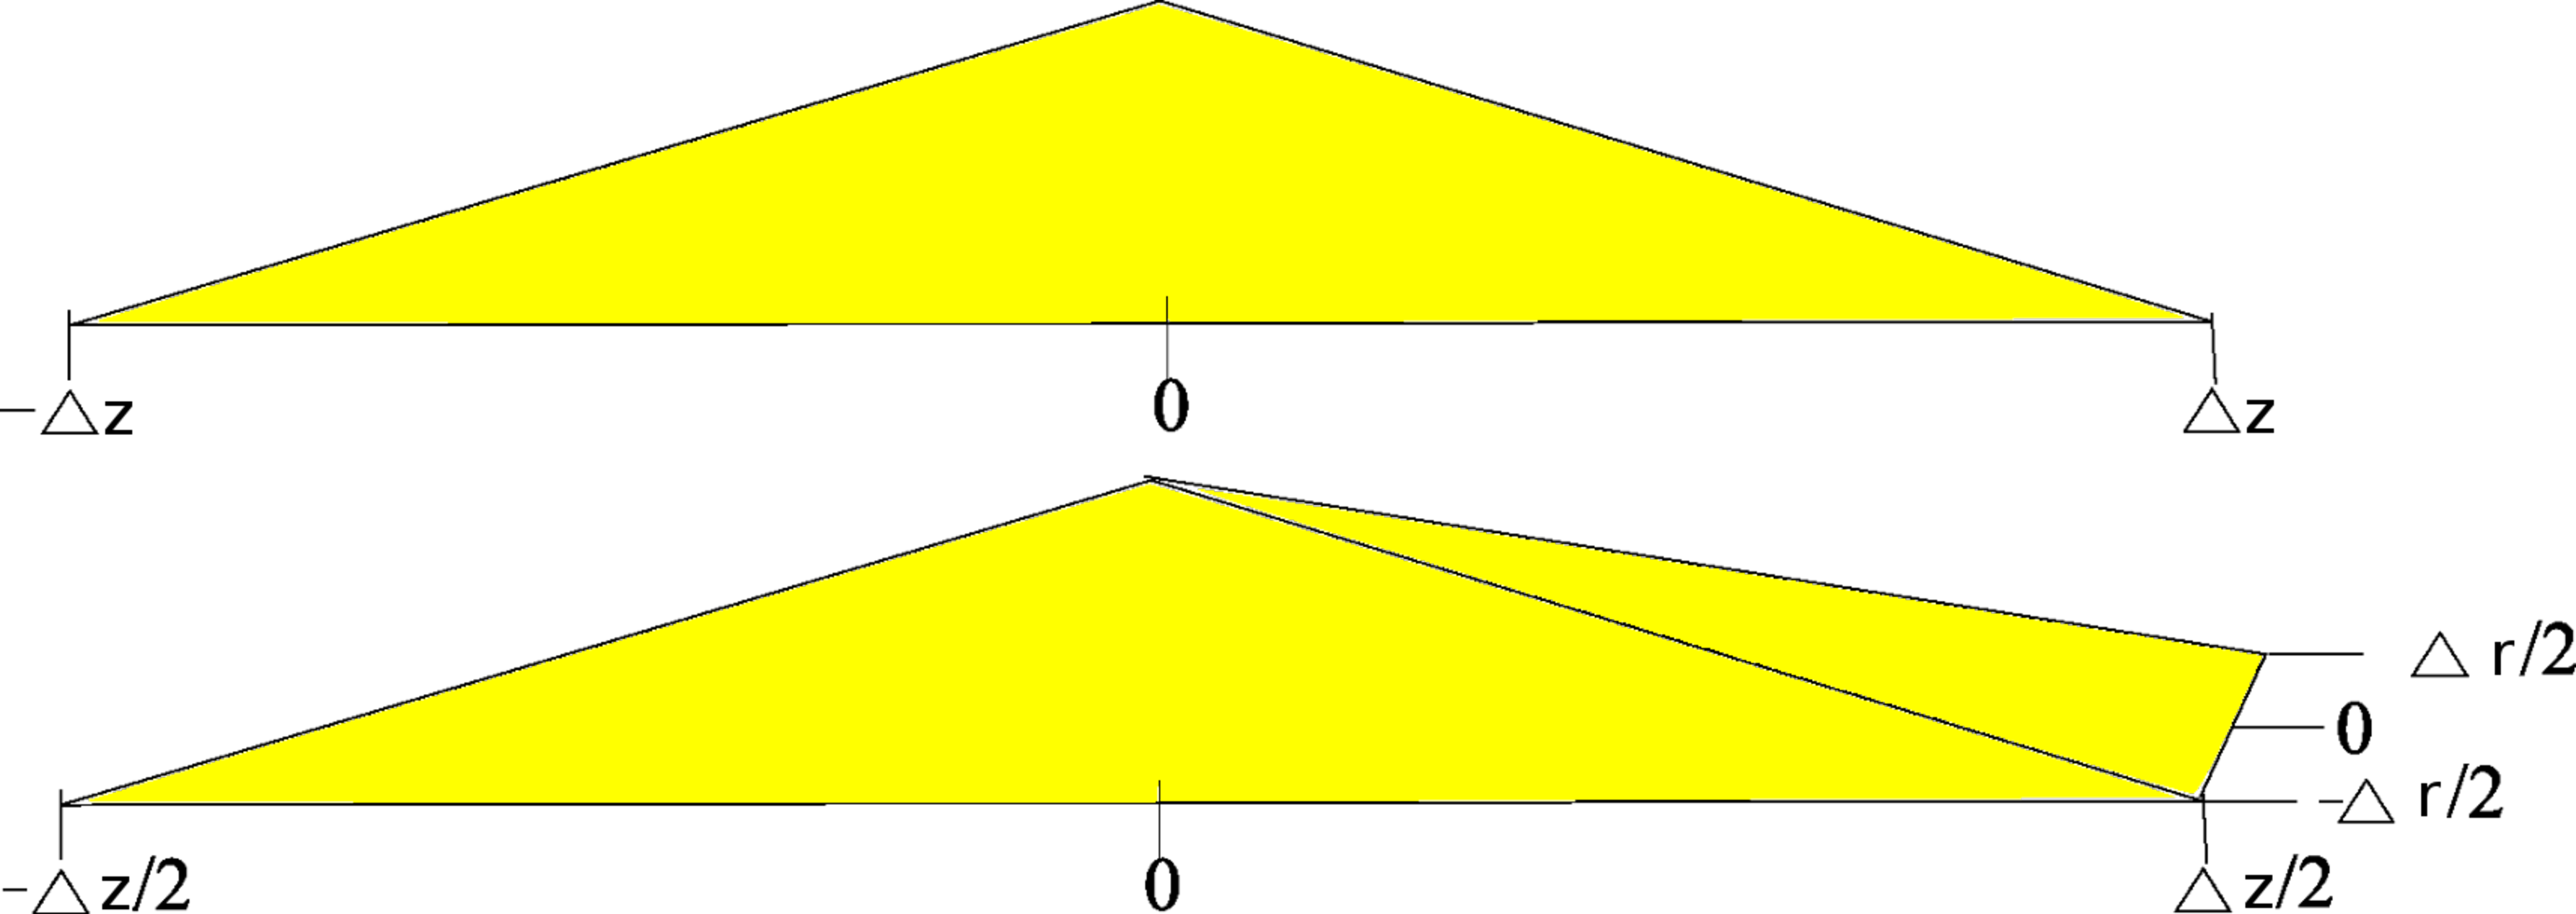
\includegraphics[width=0.8\textwidth]{figures/cicweighting.pdf}
				\caption{%
					Linear weighting scheme for (top) 1D and (bottom) 2D simulations. The latter is an expansion into the radial dimension from a 1D case. The twodimensional approximation is called Cloud-In-Cell (CIC).%
			}\label{fig:cicweighting}
			\end{figure}
%
			\begin{align}
				\text{1D:}\quad\quad\,\,\,\,%
					n\ix{j}&=\frac{S\ix{j}}{\Delta z}\left(z\ix{j}-z\right)%
					\label{equ:cicweighting1d}\\[0.0cm]
				\text{2D:}\quad\quad%
					n\ix{k,j}&=\frac{S\ix{k,j}}{A^{2}\ix{k,j}}%
					\left(r\ix{k+1}-r\right)\cdot\left(z\ix{j+1}-z\right)%
					\label{equ:cicweighting}
			\end{align}
%
			To avoid possible self-forces and satisfy the conservation of momentum, the same weighting method has to be used when back-mapping the calculated forces from the discrete grid points to the particle positions. Again, for a more detailed discussion see~\cite{Tskhakaya}.\\
			The discretised matrix equation of~\autoref{equ:fivepointstar}, and~\autoref{equ:poissonpotential} respectively, is solved using a \emph{LU-factorization}. For example, another method of matrix-solver would be the successive-over-relaxation (SOR). The potential is calculated every time step using this factorization, but the latter is done only once at the beginning, because it only depends on the mesh, and hence the composition of the matrix $\Phi\in\mathbb{R}^{N\ix{r}\times N\ix{z}}$. This is also the moment to apply any potential boundary conditions, such as external voltages $U\ix{rf}(t)$ or ground $\Phi=0$.\\
			The force resulting from~\autoref{equ:efieldmaxwell} is again mapped back to the individual particle positions using the same scheme as~\autoref{equ:cicweighting} for the, with $\Delta r\ix{0}$ equally composed 2D-mesh. Therefore, momentum conservation is satisfied.
%
			\paragraph{Particle Pusher}
%
